% !TEX TS-program = pdflatex
% !TEX encoding = UTF-8 Unicode

% This is a simple template for a LaTeX document using the "article" class.
% See "book", "report", "letter" for other types of document.

\documentclass[11pt]{article} % use larger type; default would be 10pt

\usepackage[utf8]{inputenc} % set input encoding (not needed with XeLaTeX)

%%% Examples of Article customizations
% These packages are optional, depending whether you want the features they provide.
% See the LaTeX Companion or other references for full information.

%%% PAGE DIMENSIONS
\usepackage{geometry} % to change the page dimensions
\geometry{a4paper} % or letterpaper (US) or a5paper or....
% \geometry{margin=2in} % for example, change the margins to 2 inches all round
% \geometry{landscape} % set up the page for landscape
%   read geometry.pdf for detailed page layout information

\usepackage{graphicx} % support the \includegraphics command and options
% \usepackage[parfill]{parskip} % Activate to begin paragraphs with an empty line rather than an indent

%%% PACKAGES
\usepackage{booktabs} % for much better looking tables
\usepackage{array} % for better arrays (eg matrices) in maths
\usepackage{paralist} % very flexible & customisable lists (eg. enumerate/itemize, etc.)
\usepackage{verbatim} % adds environment for commenting out blocks of text & for better verbatim
\usepackage{subfig} % make it possible to include more than one captioned figure/table in a single float
\usepackage{mathtools}
\usepackage{amsthm}
\usepackage[english,italian]{babel}
% These packages are all incorporated in the memoir class to one degree or another...

%%% HEADERS & FOOTERS
\usepackage{fancyhdr} % This should be set AFTER setting up the page geometry
\pagestyle{fancy} % options: empty , plain , fancy
\renewcommand{\headrulewidth}{0pt} % customise the layout...
\lhead{}\chead{}\rhead{}
\lfoot{}\cfoot{\thepage}\rfoot{}


%%% SECTION TITLE APPEARANCE
\usepackage{sectsty}
\allsectionsfont{\sffamily\mdseries\upshape} % (See the fntguide.pdf for font help)
% (This matches ConTeXt defaults)

%%% ToC (table of contents) APPEARANCE
\usepackage[nottoc,notlof,notlot]{tocbibind} % Put the bibliography in the ToC
\usepackage[titles,subfigure]{tocloft} % Alter the style of the Table of Contents
\renewcommand{\cftsecfont}{\rmfamily\mdseries\upshape}
\renewcommand{\cftsecpagefont}{\rmfamily\mdseries\upshape} % No bold!


%%% END Article customizations


\title{Il Gioco di Carte UNO\\Progetto del Corso di Sistemi Distribuiti\\A.A. 2016/2017}
\author{Angelo De Lisa, Alessio Netti \\ \\ angelo.delisa@studio.unibo.it\\ alessio.netti@studio.unibo.it}
\date{} % Activate to display a given date or no date (if empty),
         % otherwise the current date is printed 

\begin{document}
\maketitle
\begin{otherlanguage}{english}
\begin{abstract}
UNO è un gioco di carte multiplayer in cui l'obiettivo, per ottenere la vittoria, è quello di scartare tutte le carte della propria mano, 
prima degli avversari. Il progetto realizzato consiste nell'implementazione di una versione distribuita del famoso gioco di carte UNO, nella quale vengono 
adottate le stesse regole della versione ufficiale del gioco.
Inoltre, per garantire la continuazione della partita in corso, è stato implementato un sistema di rilevamento e riparazione del crash dei giocatori. 
In tal modo, anche se uno o più giocatori abbandonano la partita in seguito ad un crash, i giocatori restanti sono in grado di proseguire e terminare 
la partita corrente. In questo documento, dunque, vengono descritte le scelte progettuali e le varie problematiche affrontate nella realizzazione dell'applicazione.
\end{abstract}
\end{otherlanguage}

\pagebreak

\tableofcontents

\pagebreak

\section{Introduzione}
UNO è un gioco di carte in cui il numero di giocatori può variare da 2 a 8. L'obiettivo del gioco è quello di scartare, per primo, tutte le carte nella 
propria mano per ottenere la vittoria. 
Il mazzo è composto da 108 carte e prevede carte normali, alle quali è associato un numero (da 0 a 9) e un colore (blu, giallo, rosso, verde), e carte speciali
che consentono di attivare effetti particolari. Tra le carte speciali, abbiamo:
\begin{itemize}
 \item la carta ``\emph{Blocco}'': fa saltare un turno al giocatore successivo nel senso di gioco;
 \item la carta ``\emph{Cambio giro}'': inverte il senso di gioco, cioè l'ordine dei turni dei giocatori;
 \item la carta ``\emph{Pesca 2}'': il giocatore successivo nel senso del gioco pesca due carte e salta il turno;
 \item la carta ``\emph{Pesca 4}'': il giocatore successivo nel senso del gioco pesca quattro carte e salta il turno. Inoltre, consente al giocatore che l'ha
 giocata, di cambiare il colore del gioco; 
 \item la carta ``\emph{Cambia colore}'': permette al giocatore di scegliere uno tra i quattro colori disponibili come colore di gioco.
\end{itemize}
In particolare, alle carte \emph{Blocco}, \emph{Cambio giro} e \emph{Pesca 2}, è associato un colore mentre le altre due carte speciali (\emph{Pesca 4} e 
\emph{Cambia colore}) non hanno alcun colore associato.\\
Per iniziare il gioco, il mazziere distribuisce sette carte ad ogni giocatore e il mazzo restante viene
messo al centro per consentire ai giocatori di pescare quando, durante il proprio turno, nella propria mano non si hanno carte da poter scartare. 
Inoltre, da questo mazzo, viene voltata una carta che andrà a formare il cosiddetto ``\emph{mazzo degli scarti}''. 
Un giocatore può scartare una carta dalla propria mano solamente quando questa è compatibile con l'ultima carta del mazzo degli scarti. 
Compatibile significa che la carta nella propria mano è dello stesso colore o dello stesso tipo di quella in cima
al mazzo degli scarti, oppure è una carta ``\emph{Pesca 4}'' o ``\emph{Cambia colore}'', che può essere sempre giocata.\\
L'obiettivo di questo progetto è la realizzazione di una versione distribuita del gioco di carte UNO che sia utilizzabile, tramite un'interfaccia grafica 
piacevole, su più macchine differenti interconnesse tra loro. In particolare, è stata posta l'attenzione sulla tolleranza ai crash delle macchine coinvolte.
Infatti, il gioco continua la sua normale esecuzione nel caso in cui un giocatore abbandoni prematuramente la partita oppure la sua macchina vada in crash.\\
Il resto del documento si articola come segue: verrà data una panoramica del gioco nella Sezione 2; nella Sezione 3, verranno presentati gli aspetti implementativi;
il documento si conclude con possibili miglioramenti e considerazioni finali.

\section{Panoramica del Gioco}
In questa Sezione, vengono descritti il funzionamento del gioco e le varie problematiche affrontate.

\subsection{Descrizione del Gioco}
L'architettura dell'applicazione realizzata è di tipo distribuito. L'unica forma di centralizzazione utilizzata è quella che consente la registrazione dei 
partecipanti al gioco. In questo scenario, uno dei giocatori sceglie di essere l'entità centrale semplicemente spuntando la casella presente nel pannello 
di registrazione. Successivamente, una volta indicato il proprio username e il numero di partecipanti alla partita, viene inizializzato lo stato del gioco e
avviata l'interfaccia. In tale schermata, è, inoltre, presente l'indirizzo IP al quale gli altri peer devono connettersi per poter partecipare alla 
partita appena avviata. Quindi, i restanti giocatori dovranno inserire nell'apposito campo ``IP Host'', l'indirizzo IP dell'host. Tale termine deriva dal gergo relativo all'online gaming, in cui per \textit{host} si intende il giocatore che \textit{ospita} e coordina la partita. Ogni volta che un peer si
connette alla partita, l'interfaccia di gioco viene aggiornata mostrando i giocatori attualmente connessi. Quando tutti i giocatori hanno effettuato la 
registrazione alla partita, la fase di registrazione termina e nessun peer fungerà da entità centrale. Da quel momento in poi, le comunicazioni avverranno 
solamente in maniera peer-to-peer.\\
Finita la fase di registrazione, quindi, comincia la fase di gioco. Il giocatore che fungeva da host centrale è il primo a giocare. Ogni giocatore deve 
attendere il proprio turno per poter giocare la sua mossa. Quando un giocatore effettua una mossa, questa viene notificata a tutti gli altri giocatori e 
sarà visibile nell'interfaccia di gioco. Tramite l'interfaccia, è possibile osservare lo stato di gioco, cioè sapere chi ha il turno, quante carte nella 
mano ha ogni giocatore e quante carte rimangono nel ``mazzo di pesca''. Durante il gioco, alcuni giocatori potrebbero abbandonare la partita oppure
la loro macchina potrebbe andare in crash. In tal caso, il giocatore viene rimosso dalla partita corrente senza avere la possibilità di ritornare in gara, 
mentre i restanti giocatori possono continuare normalmente la partita. Per decretare un vincitore, invece, ci sono due possibilità: 
o il giocatore ha terminato tutte le carte della propria mano, oppure è rimasto l'unico giocatore attivo nel tavolo di gioco. 
In tal caso, una label notificherà al giocatore la sua vittoria.

\subsection{Problematiche Affrontate}
Di seguito saranno esposte alcune problematiche affrontate nella realizzazione del gioco e come sono state risolte:
\begin{itemize}
  \item \emph{Rilevamento di un crash in tempo reale}: essendo UNO, un gioco di carte in cui il turno è posseduto esclusivamente da un giocatore per volta, e,
  data l'architettura scelta, risulta difficile ottenere le informazioni di un crash in tempo reale, senza un continuo scambio di messaggi tra i vari host.
  Per ovviare a tale impedimento, si è pensato di istanziare un timer per ogni giocatore che, ogni 40 millisecondi, interroga il proprio successore nell'anello
  per verificare se risulta attivo. Nel caso in cui sia rilevato il crash, viene avviata la procedura per la gestione del crash e permettere il normale 
  proseguimento del gioco.
  \item \emph{Mantenere lo stato di gioco aggiornato}: quando un giocatore che possiede il turno abbandona il gioco a causa di un crash, risulta necessario attribuire il turno stesso ad un altro giocatore. Tuttavia, permettendo ad ogni player di salvare l'ultimo stato di gioco corretto, quando viene rilevato il crash del 
  giocatore di turno, viene anche rispedito il messaggio contenente le informazioni dello stato di gioco corretto a tutti gli utenti ancora connessi, permettendo di riprendere la partita. Un semplice sistema di numeri di sequenza, basato sul numero di turni giocati, permette di prevenire inconsistenze nell'aggiornamento degli stati di gioco.
  \item \emph{Gestione della carta ``Cambio giro''}: data la struttura ad anello, quando viene giocata una carta ``Cambio giro'' risulta più semplice modificare
  anche il verso della circolazione dei messaggi. Quindi, lo stato di gioco contiene una variabile in grado di determinare il verso dello scambio dei messaggi
  a seconda dell'attivazione o meno della carta speciale.
\end{itemize}

\vspace{3mm}
\section{Implementazione}
Il gioco è stato realizzato utilizzando il linguaggio Java, il quale fornisce il framework \emph{RMI} per la realizzazione di applicazioni distribuite.
Nell'implementazione del gioco, è stato utilizzato il design pattern \emph{Singleton}, attraverso il quale si garantisce che di una specifica classe venga 
generata un'unica istanza, accessibile in maniera globale da ogni punto del codice.\\
Essendo UNO un gioco di carte in cui, in ogni istante, un solo giocatore possiede il turno di gioco, è risultato logico utilizzare una struttura di comunicazione
ad anello. Infatti, quando un giocatore effettua una mossa, lo comunica al giocatore successivo, il quale, a sua volta, inoltrerà il messaggio al suo successivo.
Così facendo, il messaggio attraversa tutto l'anello fino ad arrivare di nuovo al mittente del messaggio e, quindi, ogni giocatore riceve gli 
aggiornamenti dello stato di gioco.\\
Di seguito, vengono riportati i diagrammi UML e una breve descrizione delle classi implementate, divise in 3 package: \emph{UnoRMI}, contenente le classi per 
la registrazione al gioco e la comunicazione tra i peer, \emph{UnoGame}, che contiene le classi per la logica di gioco, e \emph{UnoUI}, per l'interfaccia 
grafica.

\subsection{Package UnoRMI}
Nel package \emph{UnoRMI} troviamo le classi che permettono ai peer di registrarsi nell'arena di gioco e, successivamente, comunicare tra loro per inviare 
gli aggiornamenti dello stato di gioco. Di seguito verranno descritte le classi più importanti:
\begin{figure}[h]
\centering%
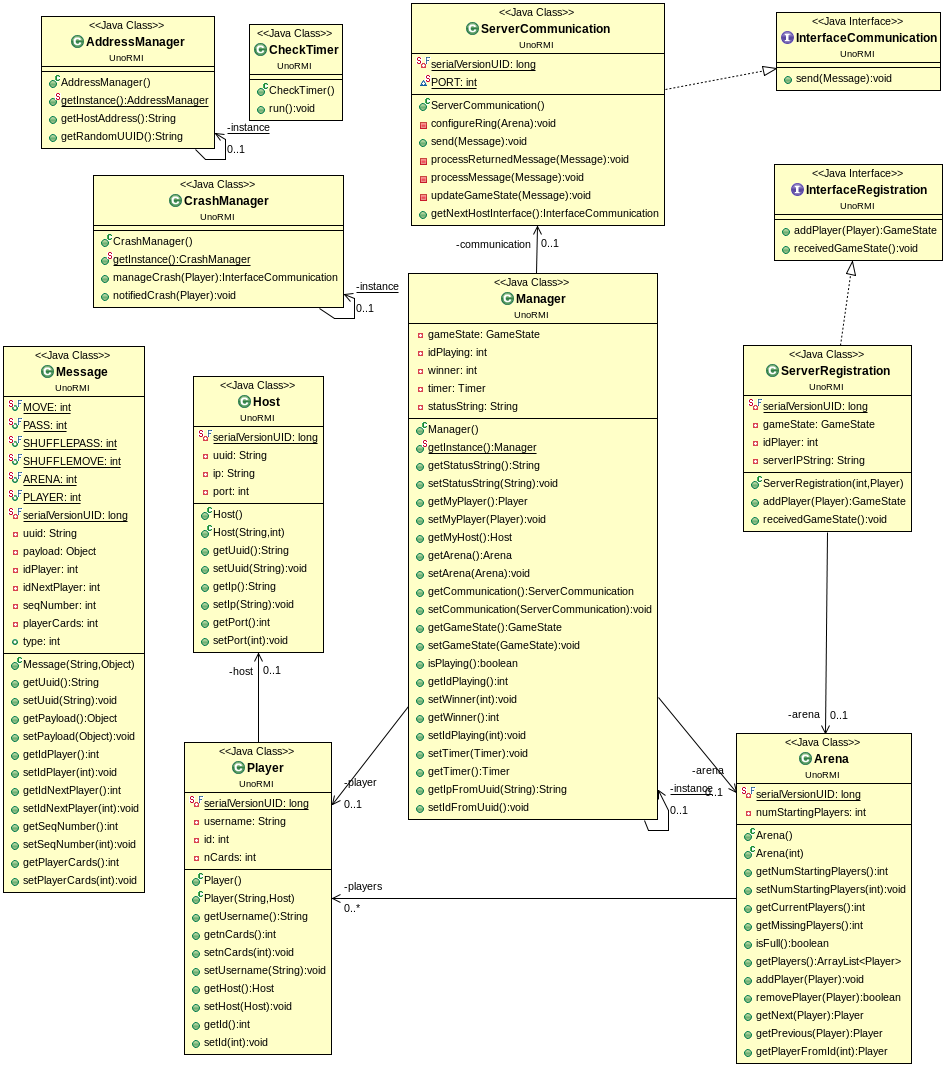
\includegraphics[height=13.5cm, width=14cm, keepaspectratio]{/home/angelo/IdeaProjects/ProgettoUnoGame/relazioneUNO/unoRMI.png}%
\caption{Diagramma delle classi del package UnoRMI.}
\end{figure}

\begin{itemize}
 \item \emph{Manager}: tale classe si occupa interamente della gestione di tutti gli aspetti del giocatore, dello stato di gioco e della comunicazione 
 con gli altri giocatori. 
 \item \emph{Arena}: classe che rappresenta l'arena di gioco alla quale i giocatori si registrano. Inoltre, tale classe contiene i dettagli di tutti i giocatori
 connessi.
 \item \emph{Player}: identifica il giocatore e tiene traccia di tutte le sue informazioni, come l'id univoco, l'indirizzo IP, l'username.
 \item \emph{Message}: rappresenta la primitiva utilizzata per la comunicazione tra i peer. Ogni messaggio inviato ha un tipo e delle variabili associate:
 \begin{itemize}
  \item MOVE: indica la mossa effettuata dal mittente del messaggio;
  \item PASS: indica che il giocatore ha passato il turno;
  \item SHUFFLEMOVE: indica che il mittente, oltre ad aver giocato una carta, ha anche rimescolato il mazzo perché il ``mazzo pesca'' era terminato;  
  \item SHUFFLEPASS: indica che il mittente, oltre ad aver passato il turno, ha anche rimescolato il mazzo perché il ``mazzo pesca'' era terminato;
  \item ARENA: viene inviato in fase di registrazione per consentire al giocatore di partecipare all'arena di gioco attiva;
  \item PLAYER: viene inviato quando un giocatore è andato in crash e, quindi, l'identità del giocatore viene comunicata a tutto l'anello per permettere 
  la rimozione del giocatore.
 \end{itemize}
 A seconda del tipo di messaggio, ogni host che lo riceve, effettua determinate azioni.
 \item \emph{ServerRegistration}: classe che implementa un servizio di registrazione centralizzato, in remoto, dei giocatori. Si occupa, di allestire l'arena
 di gioco e di aggiungervi i partecipanti.
 \item \emph{ServerCommunication}: classe che implementa i metodi remoti necessari per la comunicazione tra i vari giocatori connessi all'arena di gioco. 
 Permette, quindi, la ricezione e l'invio dei messaggi e consente di ottenere l'interfaccia di rete del prossimo host al quale inoltrare il messaggio.
 \item \emph{CrashManager}: si occupa di gestire i crash che avvengono durante una partita, provvedendo ad eliminare i giocatori non connessi e a notificare
 i restanti giocatori dell'avvenuto crash.
\end{itemize}

\subsection{Package UnoGame}
Il package UnoGame include tutte le classi destinate all'implementazione della logica di gioco effettiva. Troviamo, dunque, tutte le classi necessarie per la rappresentazione degli oggetti di gioco, delle relative regole, nonché per l'aggiornamento dello stesso. In particolare, il package si compone delle seguenti classi:
\begin{figure}[h]
\centering%
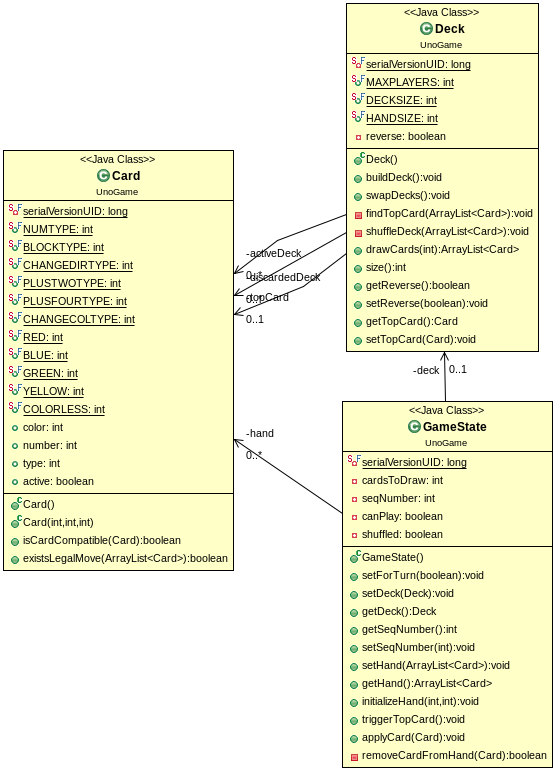
\includegraphics[height=13.5cm, width=14cm, keepaspectratio]{/home/angelo/IdeaProjects/ProgettoUnoGame/relazioneUNO/UnoGame.png}%
\caption{Diagramma delle classi del package UnoGame.}
\end{figure}

\begin{itemize}
	\item \emph{Card}: questa classe codifica il più semplice oggetto di gioco, ossia la \textit{carta}. Tale oggetto è identificato da un valore numerico ed un tipo, dipendenti dalla specifica carta. La classe, inoltre, implementa metodi per determinare se una carta può essere giocata su di un'altra, realizzando gran parte delle regole di gioco.
	\item \emph{Deck}: tale classe implementa il \textit{mazzo} di gioco, che si compone di tre elementi, ossia il mazzo di carte pescabili, il mazzo di carte scartate, ed infine la carta attualmente attiva, rispetto alla quale vanno effettuate mosse. Tale classe realizza anche metodi per l'inizializzazione ed il mescolamento del mazzo, nonché per l'estrazione di carte. 
	\item \emph{GameState}: Il GameState codifica lo stato attuale del gioco dal punto di vista di un singolo giocatore. Essa include, di conseguenza, il Deck di gioco attuale (uguale per tutti i giocatori) e la \textit{mano} del giocatore, realizzata come \textit{collezione} di oggetti Card. Sono presenti, inoltre, alcune variabili atte a semplificare la gestione del turno. Altre variabili relative alla gestione del gioco, come l'ID del giocatore che attualmente detiene il turno oppure l'ID del vincitore, sono gestite dalla classe Manager in modo da semplificarne la manipolazione, in questo caso maggiormente legata all'oggetto Arena attuale.
\end{itemize} 

\subsection{Package UnoUI}
Nel package UnoUI possiamo ritrovare la realizzazione dell'interfaccia di gioco. Essa consta di due componenti principali: una interfaccia di configurazione iniziale, realizzata tramite la libreria Java Swing, e l'interfaccia di gioco effettiva, realizzata in OpenGL per mezzo della libreria LibGDX. Le classi ritrovabili all'interno del pacchetto sono le seguenti:
\begin{figure}[h]
\centering%
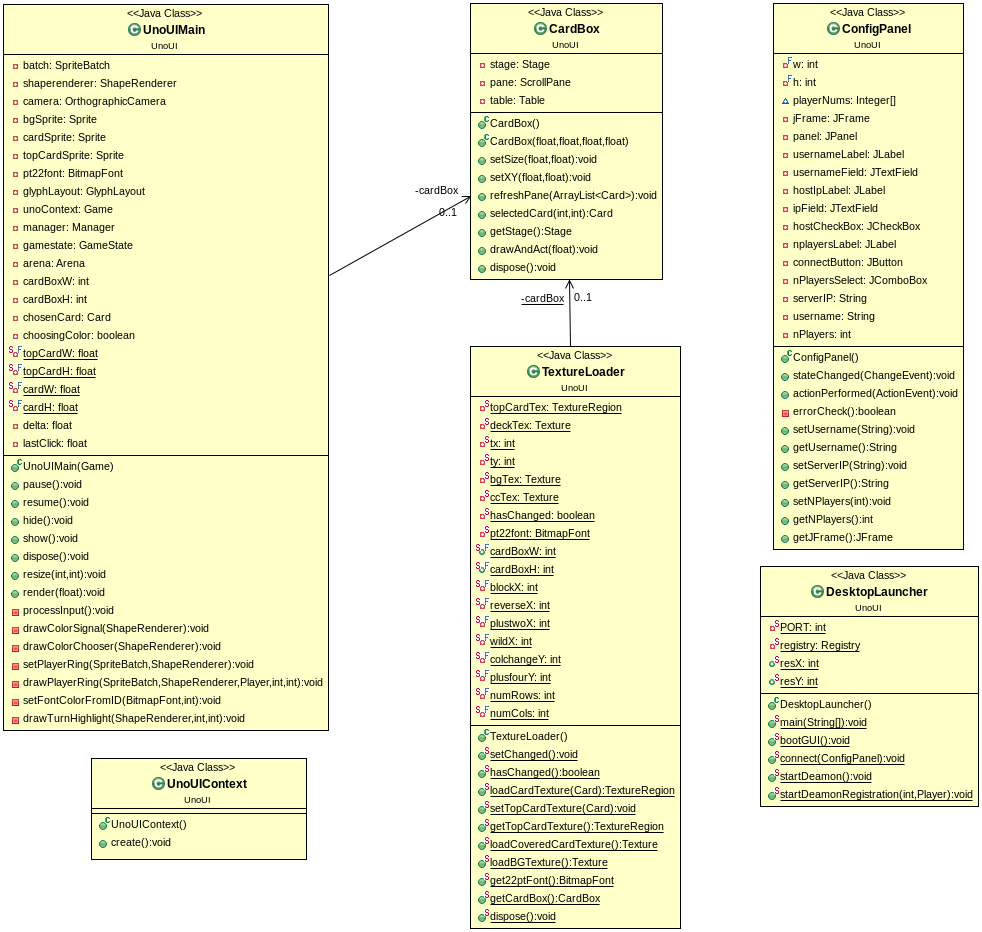
\includegraphics[height=13.5cm, width=14cm, keepaspectratio]{/home/angelo/IdeaProjects/ProgettoUnoGame/relazioneUNO/UnoUI.png}%
\caption{Diagramma delle classi del package UnoUI.}
\end{figure}
\begin{itemize}
	\item \emph{DesktopLauncher}: in questa classe è implementato il metodo \textit{main} atto all'avvio dell'intera applicazione. Essa si occupa dunque di avviare l'interfaccia di configurazione, e successivamente di procedere alla connessione con la macchina \textit{host} ed all'avvio dell'interfaccia di gioco.
	\item \emph{ConfigPanel}: tale classe implementa l'interfaccia di configurazione iniziale, realizzata tramite la libreria Swing di Java. Essa presenta due \textit{fields} testuali per l'inserimento dell'username e dell'indirizzo IP relativo alla macchina Host della partita, oltre ad un \textit{checkbox} utilizzato nel caso in cui si voglia impersonare tale ruolo. Infine, è presente un menu a tendina per la selezione del numero di giocatori, attivato solo nel caso in cui si scelga di fungere da Host per la partita.
	\item \emph{UnoUIMain}: classe che realizza l'interfaccia di gioco vera e propria, realizzata tramite la libreria LibGDX, basata su OpenGL. Differentemente dall'uso di Swing, in cui il ri-disegno avviene soltanto su richiesta, in questo caso troviamo un metodo \textit{render}, richiamato automaticamente ad intervalli regolari in modo da realizzare una interfaccia fluida e reattiva. La gestione dell'input utente avviene in questa stessa classe, internamente al metodo \textit{render}.
	\item \emph{UnoUIContext}: si tratta di una classe di gestione del \textit{contesto} OpenGL, istanziata all'avvio dell'applicazione, ma non realmente utilizzata, seppur necessaria.
	\item \emph{CardBox}: implementa il \textit{box} scrollabile posto nella parte inferiore dell'interfaccia, che rappresenta l'insieme di carte appartenenti alla mano del giocatore. Essa realizza tutti i metodi per il rendering, l'aggiornamento e l'interazione con tale parte dell'interfaccia.
	\item \emph{TextureLoader}: classe che si occupa della gestione statica di tutte le risorse grafiche, tra cui textures e fonts, che vengono allocate una sola volta, e poi riutilizzate in parti differenti dell'applicazione. Tale classe si basa sul design pattern \textit{singleton}, e permette un più efficiente utilizzo della memoria grafica. 
\end{itemize}

\vspace{3mm}
\section{Conclusioni}
In questo documento, è stato descritta l'implementazione di una versione distribuita del gioco di carte UNO. Tramite la struttura ad anello e 
lo scambio dei messaggi, ogni giocatore è aggiornato in tempo reale sullo stato di gioco. 
Inoltre, grazie alla gestione dei crash, ogni giocatore ancora connesso è in grado di continuare indisturbato
la propria sessione di gioco fino al termine della partita. Sono state gestite anche situazioni di errore particolari, ad esempio quando ad abbandonare
la partita è proprio il giocatore che possiede il turno. In tal caso, lo stato della partita non viene alterato e il gioco continua normalmente. 
Riassumendo, l'applicazione è in grado di tollerare \emph{n-1} guasti (con \emph{n}=numero di giocatori). In questo modo, la partita rimane attiva finchè è 
connesso almeno un giocatore, il quale, però, sarà decretato vincitore della partita in quanto l'unico attivo nell'arena di gioco.\\
Come possibile ulteriore sviluppo, si potrebbe migliorare l'interfaccia del pannello di registrazione.
L'interfaccia grafica di gioco, invece, risulta essere piacevole e intuitiva e non richiede particolari raffinamenti.  
\end{document}

